%!TEX root = ../thesis.tex
% 2 - Advanced Concepts

\chapter{Fundamental concepts about spectroscopy and RV}
\label{cha:concepts}
In this chapter we will expand  on the RV section and nir spectroscopys. Follwing that we will  detail the synthetic spectral models used in the work. both of PHOENIX aCES btsettl and tapas 


To put things too detailed for the introduction?


Spectrograph design stuff




Radial Velocity:
Picture of orbital motion.
Concepts of {RV} motion-
Masses,
Orbits, (period, mass, distance impact.)
Equation
What the Equations mean.
\begin{figure}
    \centering
    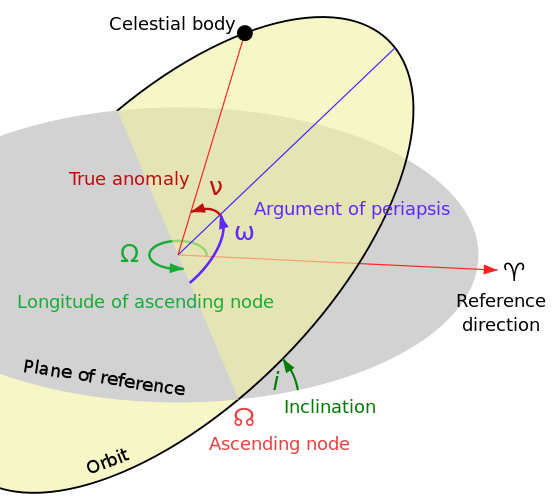
\includegraphics[width=0.7\linewidth]{figures/advanced_material/orbit}
    \caption{By Lasunncty at the English Wikipedia, CC BY-SA 3.0, \href{https://commons.wikimedia.org/w/index.php?curid=8971052}{https://commons.wikimedia.org/w/index.php?curid=8971052}}
    \label{fig:orbit}
\end{figure}

{ }

\subsection{{RV} calculation}
\unfinished{Move location / adjust from paper}
We use the Keplerian orbit {RV} equation to estimate the {RV} of the host and companions at the time of each observation, \(t\):
\begin{equation}
\label{eq:rv_equation}
{RV} = K [\cos{(\nu(t) + \omega)} + e\cos{(\omega)}]
\end{equation}
Here, \emph{K} is the \emph{semi-major amplitude}, \(\nu\) is the \emph{true anomaly}, \(e\) is the orbital \emph{eccentricity}, and \(omega\) is the \emph{argument of periastron}.
The true anomaly is not only a function time, \(t\), but also the orbital period \(P\), the \emph{time of periastron passage}, \(T_0\), and eccentricity.
The literature parameters for each target are provided in \tref{tab:orbitparams}.
To determine the {RV} of the companion we transformed the {RV} semi-amplitude of the host \(\kone\) into the semi-amplitude for the companion \(\ktwo\) using the mass ratio,
\begin{equation}
\label{eqn:mass_ratio}
q = \mtwo / \mone = \kone / \ktwo
\end{equation}

We note that for the targets in which only the minimum mass (\mtwosini) is known, this equation will indicate the maximum \(\ktwo\) value for the companion. The estimated \(\ktwo\) for each companion is provided in \tref{tab:estimatedparameters} while the {RV} for both components at the time of each observation is provided in \tref{tab:observations}.

The error on estimated {RV} values, shown in \fref{fig:HD211847_result_contours} is calculated by applying the general error propagation formula~\citep{ku_notes_1966} and using the  errors on the orbital parameters. For a function, \(f\), with errors on the inputs \(\delta x\), \(\delta y\) etc., it follows:
\begin{align}
f &= f(x, y, z, \ldots)\\
\delta f &= \sqrt{{\left( \frac{\partial f}{\partial x} \delta x\right)}^2 + {\left(\frac{\partial f}{\partial y} \delta y\right)}^2 + {\left(\frac{\partial f}{\partial z} \delta z\right)}^2 + \ldots}
\end{align}

\section{Estimating Companion-host Flux ratio}
\label{sec:compaion_flux_ratio}
In order to visually or spectroscopically detect binary or planetary companions it is helpful to calculate the flux/contrast ratio between the host and companion.

The companion-host flux or contrast ratio of the system can be estimated using:
\begin{equation}
\frac{F_{2}}{F_{1}} \approx 2.512^{m_{1} - m_{2}}, \label{eqn:mag_flux_ratios}
\end{equation}
where \(m_{1}\) and \(m_{2}\) are the magnitude of the host and companion respectively.

The photometric apparent magnitudes for the host stars, \(m_{1}\), in several wavelength bands are easily obtained online catalogues such as {SIMBAD}~\citep{wenger_simbad_2000} or {2MASS} \citep{skrutskie_two_2006}.
However, the magnitudes of the companions, \(m_{2}\), are not readily available as they have not been directly measured.
To estimate the magnitude of the companions stellar evolution models of \citet{baraffe_evolutionary_2003, baraffe_new_2015} are used.
These models tabulate several properties of low-mass stars and BDs during their evolution.
These include the temperature, radius, luminosity, and absolute magnitudes in several photometric bands, for a range of companion masses and stellar ages.
A given companion mass, and a stellar age will uniquely identify a point in the Baraffe models which corresponds to a specific magnitude for the companion.
The tables provided in \citet{baraffe_evolutionary_2003, baraffe_new_2015} are also interpolated to reach companion masses and stellar ages between the models provided.

In \tref{tab:estimated_flux_ratios} the host-companion flux ratio estimates for the targets analysed in this work are presented. The {K}-band flux ratios are calculate as the observed spectra are in the {K}-band at 2.1\um{}. The ages for the stellar system used are given in \tref{tab:starparams} while the companion masses are given from \tref{tab:orbitparams}. These both are used to obtain the absolute magnitude for the companions.  For the companions in which only the minimum mass (\mtwosini{}) is known then the flux-ratio given will be the lower limit, or worst case scenario.

%!TEX root = ../../thesis.tex
\begin{table*}
    \small
    \centering
    \begin{threeparttable}[b]
        \caption{Estimated flux ratios given the companion mass (\(\textrm{M}_{2}\) or \(\textrm{M}_{2} \sin{i}\)) from \tref{tab:orbitparams}.} 
        \begin{tabular}{l c c c c c c}%[hb]
            \toprule
            & Host& & Host & Companion & Estimated & Estimated  \\  % 2017
            Companion & $m_{K}$ & $\pi$ & M\(_{K}\) & M\(_{K}\) & \(\rm F_{2}/F_{1} \) & \(\rm N_{2}/N_{1} \) \\
            & & mas & & & \textit{K}-band &  (noise ratio) \\
            \midrule
            {HD 4747} & 5.305 & 53.184 & 3.82 & 14.17 & \(7\times10^{-5} \) & 76 \\  % 2017
            {HD 162020} & 6.539 & 32.410 & 4.10 & 23.36 & \(2\times10^{-8} \) & 1\,615 \\  %
            {HD 167665} & 5.038 & 32.014 & 2.60 & 13.21 & \(6\times10^{-5} \) & 105 \\  %  -- \(2\times10^{-5} \)  best case based on age rage.
            {HD 168443b} & 5.211 & 25.208 & 2.35 & 42.19 & \(1\times10^{-16} \) & \(1\times10^{8} \) \\ 
            {HD 168443c} & 5.211 & 25.208 & 2.35 & 29.55 & \(1\times10^{-11} \) & \(4\times10^{5} \) \\  %(c)
            {HD 202206}B & 6.485\tnote{a}& 21.726 & 3.04 & 21.63 & \(4\times10^{-8} \) & 1\,586 \\  %(B)   % May2017
            {HD 202206}c & 6.485\tnote{a}& 21.726 & 3.04 & 45.63 & \(9\times10^{-18}\) & \(2\times10^{7} \) \\  %(B)   % May2017
            {HD 211847}B & 7.018 & 20.489 & 3.50 & 8.40 & 0.011 & 14 \\  %B % 2017
            {HD 30501} & 5.525 & 49.081 & 3.96 & 10.38 & 0.003 & 27 \\
            \bottomrule
        \end{tabular}\label{tab:estimated_flux_ratios}
        \begin{tablenotes}
            \item  [a]{Magnitude from {2MASS} catalogue instead of {SIMBAD}.}
        \end{tablenotes}
    \end{threeparttable}

\end{table*} % \label{tab:estimated_flux_ratios}

The magnitudes provided by {SIMBAD} are given in apparent magnitude, $m$, while the magnitudes in the evolutionary models are absolute magnitudes $M$. That is, the apparent magnitude that the star would have if it was observed at a distance of 10 parsecs (32.6 light-years). The apparent magnitudes of the hosts are converted to absolute magnitudes using \(M = m - \mu\) where \(\mu\) is the distance modulus:
\begin{equation}
\mu = 5 \log_{10}(d_{pc}) -5. \label{eqn:distance_modulus}
\end{equation}
Here $d_{pc}$ is the distance to the object in parsec. The distance is obtained from the trigonometric parallax  $\pi$ using the formula $d(pc) = 1 /\pi(arcsec)$, with the parallax in arcseconds\footnote{Most parallax values e.g. GAIA are tabulated in milliarcseconds (mas). Therefore it is important to remember to convert the parallax to arcseconds first, to avoid embarrassing calculation errors!}. In this work the recent high-precision parallax measurements from GAIA are used  \citet{collaboration_gaia_2018}.

From the flux ratio the noise ratio between the host and companion can also calculated in a similar way using the equation \(N_{2}/N_{1} = \sqrt{2} \times\sqrt{F_{1}/F_{2}}\).

\todo{this section is completed i think}

\subsubsection{Baraffe tables}
\label{subsubsec:baraffe_tables_code}
A simple tool\footnote{Available at \url{https://github.com/jason-neal/baraffe_tables}} was created to calculate/estimate the host-companion flux ratio using the \citet{baraffe_evolutionary_2003,baraffe_new_2015} evolution tables.
Given the name of the target star, the mass of a companion and the stellar/system age it determines the flux ratios the available spectral bands.
The tool uses the targets name  to query\href{https://zenodo.org/record/1160627}{\emph{astroquery} package} the {SIMBAD} database to obtain the stellar properties, specifically the flux magnitudes and parallax. It then interpolates the Baraffe tables to the desired companion mass and age, calculating and returning values for all parameters of the companion given in the tables (e.g. \(\teff\), \logg, \(R/R_{\odot}\)).
The stellar magnitudes are converted to absolute values using \eref{eqn:distance_modulus} and the flux ratios computed using  \eref{eqn:mag_flux_ratios}.

An extension of this tool is that can be used to perform the reverse calculation also. That is, given the target name, age and flux ratio in a given band it can estimate the mass of the companion mass using the Baraffe tables.

\todo{this section is completed i think}



% from draft of paper 18/7/2017
\subsection{Companion K}  Maybe something can go above from this ...
\label{sec:companion_RV}
\emph{These sections might be unnecessary}\\

To calculate the {RV} of the companion at the time of each observation. For a two-body system the {RV} semi-amplitude of the companion \(\ktwo\) can be determined from the orbital host-companion mass ratio \[q = \mone/\mtwo = \ktwo/\kone\label{eqn:q_ratio_K2}\].
Note, that for the targets in which only the minimum mass (\mtwosini) is known, this will give the maximum {RV} semi-amplitude of the companion.
This relation was used to estimate \(\ktwo\) for the companion from the minimum mass or mass we have for each companion. These values along with the other orbital parameters of the system were use to calculate the {RV} of the companions for each observation. These values are provided with the observations in \tref{tab:observations}.




\section{Telluric correction}


\subsection{Telluric models}

Utilizing telluric models has been shown to be better than the standard star method.
\subsubsection{TAPAS}

\subsection{Tapas models}
\todo{ADAPT THis section to explain the models more generally. Move the usage back to Reduction section}
\label{subsec:tapas_models}
For the wavelength calibration and telluric correction methods we use telluric line models. These have been show to provide as good or better telluric correction compared to the telluric standard method \reference{telluric model correction methods original}and~\citep{ulmer-moll_telluric_2018}.

We utilized the {TAPAS} (Transmissions of the AtmosPhere for AStronomical data) web-service\footnote{\url{http://www.pole-ether.fr/tapas/}}~\citep{bertaux_tapas_2014} to obtain atmospheric transmission models for each observation. {TAPAS} uses the standard line-by-line radiative transfer model code LBLRTM~\citep{clough_linebyline_1995} along with the 2008 {HITRAN} spectroscopic database~\citep{rothman_hitran_2009} and {ARLETTY} atmospheric profiles derived using meteorological measurements from the {ETHER} data center\footnote{\url{http://www.pole-ether.fr}} to create telluric line models.

The {ARLETTY} atmospheric profiles have a 6 hour resolution, so there may be a slight difference between the actual profile at the time of observation.

We use the mid-observation time to retrieve transmission models for each observation, with the {ARLETTY} atmospheric profiles\footnote{Nearest of the 6 hourly profiles} and vacuum wavelengths selected. The telluric models were retrieved without any barycentric correction to keep the telluric lines at a radial velocity of zero with respect to the instrument.

{TAPAS} allows for the choice of atmospheric constituents included in the model spectra. We obtained one model with all available species present, convolved to a resolution of \(\rm R=50\,000\), and another two models without an instrumental profile convolution applied. For these two extra models, one contained only the transmission spectra of \ce{H2O}while the other contained all other constituents except \ce{H2O}. This was to explore a known issue with the depth of \ce{H2O}absorption lines in the TAPAS~\citet{bertaux_tapas_2014}. \sref{subsec:telluric_correction}.


\todo{Look at} -> synthesizing telluric spectra \nir{} for {CRIRES}~\cite{seifahrt_synthesising_2010}

Using {TAPAS} is contrasted alongside Molecfit and Telfit in~\cite{ulmer-moll_telluric_2018}. We conclude that \ldots







%!TEX root = ../../thesis.tex


\section{Synthetic Stellar models of cool stars}
Modelling of stellar structure, atmospheres and evolution is used to try and understand the observations, pieced together with several physical, chemical and hydrodynamical models.
One output from these models is synthetic stellar spectra.
These spectra can be compared to observed spectra to attempt to classify and understand the stellar populations.
There is an ever evolving effort to improve these stellar models and synthetic spectra to better match the observations; incorporating more physics, chemical reactions and line lists, and using the latest element abundances.
In this work extensive use of the {PHOENIX-ACES} models is made with some experimentation with the {BT-Settl} models.
A collection of several theoretical stellar spectral libraries can be found at the Spanish Virtual Observatory \href{http://svo2.cab.inta-csic.es/theory/newov/index.php}{Theoretical Spectra Web Server}.

The~\citet{kurucz_model_1979} models are popular synthetic models for stars ranging between G-O type with effective temperatures between 5500--50\,000\K{}.
For cooler stars, M-dwarfs and even Brown Dwarfs the stellar models are based on the {PHOENIX} code~\citep[e.g.][]{hauschildt_parallel_1997}.
Initially created for studying the ejecta of Novae it was \emph{Extended} to low mass stars and Brown Dwarfs~\citep{allard_model_1995}.
The {PHOENIX} modelling code has evolved over time incorporating new physical models to better explain the atmospheres.
The \emph{NextGen} models~\citep{hauschildt_nextgen_1999} treated the stellar atmosphere as a gas in chemical equilibrium, but the resulting spectra for very low mass stars was poor due to no treatment of dust in the stellar atmospheres.

The~\citet{allard_limiting_2001} \emph{COND} and \emph{DUSTY} models both investigate the extreme limits of clouds in the atmospheres of cool stars.
They include condensation physics (Gibbs free energy, gas partial pressures etc.) into the chemical equilibrium model, as well as the optical interaction of light with the dust/condensates (dust opacities and scattering).
The \emph{DUSTY} models simulate `inefficient/no settling' where condensation/dust forms and stays in the atmosphere and it affects the spectrum through the dust opacities.
At the other extreme the \emph{COND} models ignore the dust opacities and simulate `efficient settling', in which all the condensates and dust clouds fall below the spectrum forming region.

The treatment of clouds and dust is important for the modelling of low mass stars and Brown Dwarfs.
The \emph{DUSTY}/\emph{COND} models are similar above 2600\K{} but below this temperature they diverge due to the crystallization of silicates in the atmosphere~\citep{allard_limiting_2001}.
These are only a few of the physical considerations implemented in the synthetic models.
The other notable changes in the name convention for the synthetic spectra are due to use of specific line lists.
The models beginning with {AMES} use the {NASA-AMES} \ce{H2O} and \ce{TiO} line lists, while the {BT} models use the~\citet{barber_highaccuracy_2006} \ce{H2O} line list.
Between models the use of improved solar abundance measurements is also included~\citep[][]{asplund_chemical_2009}.

In this work synthetic spectral from the {PHOENIX-ACES} and to a lesser extent the {BT-Settl} stellar models are used.
These are further evolutions of the \emph{DUSTY}/\emph{COND} models and are detailed below.

Both sets of synthetic models do not handle the affects of radiation from a neighbouring star, which may have an affect on the BD companions studied here.

\subsection{{PHOENIX-ACES} models}
\label{subsec:phoenix_aces}

The {PHOENIX-ACES} models~\citep{husser_new_2013} are a descendant of the \emph{COND} models.
They include condensation in equilibrium with the gas phase while ignoring dust opacity and any mixing or settling which is important for cooler atmospheres.
As such the {PHOENIX-ACES} models are restricted to \Teff{}>2300\K{} as the treatment of dust/clouds is not handled.
It uses the most recent version (16) of the {PHOENIX} code and is suitable for the spectra of cool stars.
THE {PHOENIX-ACES} models uses the Astrophysical Chemical Equilibrium Solver (ACES, Barman 2012) new in version 16 of {PHOENIX} to perform state-of-the-art treatment of the chemical equilibrium.
It also adds parametrisations for the mass and mixing-length, and uses the solar abundances of~\citet{asplund_chemical_2009}.

As noted in~\citep{husser_new_2013} there are significant differences between the spectra from {PHOENIX-ACES} and previous {PHOENIX} model spectra.
For instance the equation of state solver ACES strongly affects the stellar structure and different line and molecular band strengths.
Unfortunately there are several changes introduced with {PHOENIX-ACES} making it difficult to distinguish and quantify the different effects.

The full parameter grid space of the pre-computed {PHOENIX-ACES} spectra is given in \cref{tab:phoenix} although this full range is not utilized in this work.
This work uses models below >7000\K{} with no \(\alpha\) variation\footnote{$\alpha$ elements are created during nuclear fusion by the successive addition of helium nuclei (alpha particles), thus have atomic numbers with an integer multiple of 4.}.
The spectral sampling of the grid are $R \approx 50\,000$ for 300--2500\nm, covering the wavelengths used here.

%!TEX root = ../../thesis.tex

\begin{table}
    \centering
    \caption{Full parameter space of the {PHOENIX-ACES} spectral grid. Reproduced from~\citet{husser_new_2013}.}
    \begin{tabular}{cr@{ -- }lc}    % Seperate columns with --
        \toprule
         & \multicolumn{2}{c}{Range}       & Step size\\
        %\midrule
        \midrule
        \multirow{2}*{\txteff{} [K] }  &  2\,300 & 7\,000    & 100 \\
                                                          &  7\,000 & 12\,000  & 200 \\ 
        \logg{}                                      &  0.0      & +6.0       & 0.5 \\
        \multirow{2}*{\feh{}}            &  -4.0     & -2.0        & 1.0 \\    % Strange spacing of [ ] in table so added \ to all rows
                                                         &  -2.0     & +1.0       & 0.5 \\
        \(\alpha\)/Fe                              &  -0.2     & +1.2       & 0.2 \\
        \bottomrule
    \end{tabular}
    \label{tab:phoenix}
\end{table}

\todo{Use multirow}

The lower temperature limits of this library limits the stellar mass to the high mass BDs.
For example a \Teff{}=2300\K{} corresponds to a {BD} with \(\textrm{M}\sim84\)\Mjup{} at 5\Gyr{} from the~\citet{baraffe_evolutionary_2003} evolutionary models, (see \cref{sec:evolutionary_models}).


While using the {PHOENIX-ACES} models a discontinuity in the stellar flux is observed between 5000\K{} and 5100\K{}.
In \cref{fig:phoenixdiffereceat5000k} several {PHOENIX-ACES} spectra in incremental steps are shown in a small wavelength range of 2113--2115\nm{}.
The line profile seems to change suddenly between the model with 5000\K{} and 5100\K{}, causing a slight discontinuity in the models.
This slightly impacts the use of these models while attempting \textchisquared{} fitting in \cref{cha:model_comparison}.
The bottom panel shows the flux difference between models separated in temperatures of 100\K{} (one grid step).
The difference between 5000 and 5100\K{} (green) is offset from the other model differences.
This is potentially caused by the change in treatment of the model atmospheres at 5000\K{}.
For instance~\citet{husser_new_2013} mention that the reference wavelength defining the mean optical depth grid, is fixed to $\lambda_{\tau}=1200$\nm{} for \Teff{}>5000\K{} and $\lambda_{\tau}=500$\nm{} for hotter stars in the {PHOENIX-ACES} modelling.

\begin{figure}
    \centering
    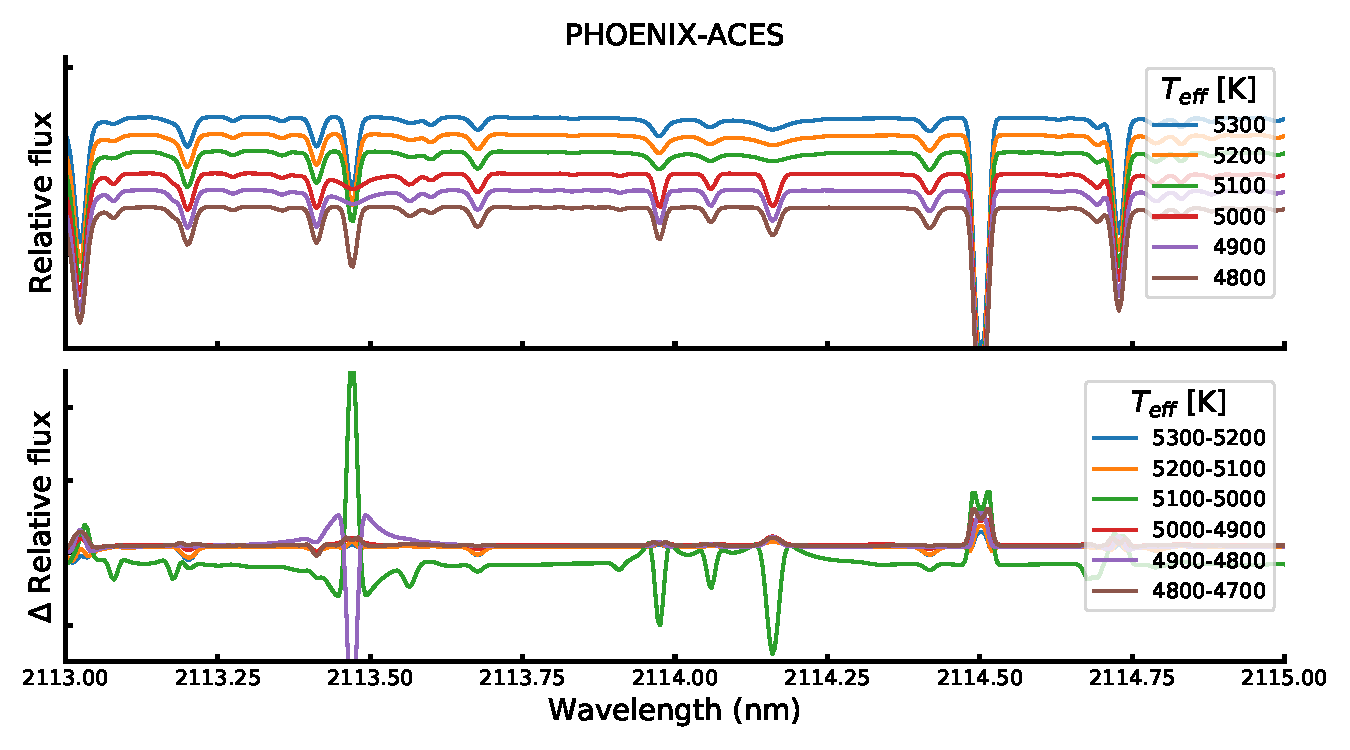
\includegraphics[width=0.7\linewidth]{figures/atmos_and_models/phoenix_differece_at_5000K}
    \caption[Difference in successive {PHOENIX-ACES} spectra around 5000\K.]{Top: Incremental {PHOENIX-ACES} model spectra between 4800--5300\K{} with \logg{}=4.5 and \feh{}=0.0 fixed.
    Bottom: Difference in flux between successive models separated by 100\K{}.
    Apart from near absorption lines there is a discontinuity in the flux of the {PHOENIX-ACES} models between 5000 and 5100\K{}.}
    \label{fig:phoenixdiffereceat5000k}
\end{figure}


\subsection{BT-Settl}
\label{subsec:btsettl}
The {BT-Settl} models~\citep{allard_models_2012,allard_atmospheres_2012,rajpurohit_effective_2013,baraffe_new_2015}, are an evolution of both the \emph{DUSTY} and \emph{COND} models.
They are better suited for the entire range of {BD} temperatures down to 400\K{}, through hydrodynamical modelling of the mixing and settling of dust/clouds in the atmosphere of cool dwarfs~\citep{freytag_role_2010}.
The {BT-Settl} models now also include 3-D radiation transfer~\citep{seelmann_3d_2010}.

The {BT-Settl} are generally more difficult to work with due to their file format (in comparison to {PHOENIX-ACES}).
The most recent {BT-Settl} spectral library designated {CIFIST2011\_2015}\footnote{\url{https://phoenix.ens-lyon.fr/Grids/{BT-Settl}/CIFIST2011_2015/}}~\citep{baraffe_new_2015} includes newer~\citet{caffau_solar_2011} solar abundances and is combined with evolutionary modelling.
It is available in a fits format which is easier to use.
They work on the version 15.5 of the {PHOENIX} code.
The parameter range available from the pre-computed library is given in \cref{tab:btsettl_params}.

%!TEX root = ../../thesis.tex

\begin{table}
    \centering
    \caption[{BT-Settl} parameter space.]{Full parameter space of the {BT-Settl} ({CIFIST2011\_2015}) spectral grid~\citet{baraffe_new_2015}.}
    \begin{tabular}{cr@{ -- }lc}    % Seperate columns with --
        \toprule
         & \multicolumn{2}{c}{Range}       & Step size\\
        \midrule
        \txteff{} [K]  &  1\,200 & 7\,000    & 100 \\
        \logg{}          &  2.5      & 5.5         & 0.5 \\
        \feh{}            & 0          & 0            & - \\    % Strange spacing of [ ] in table so added \ to all rows
        \(\alpha\)/Fe   &  0         & 0            & - \\
        \bottomrule
    \end{tabular}
    \label{tab:btsettl_params}
\end{table}


In this work the {BT-Settl} models used did not go below the {PHOENIX-ACES} limit of 2300\K{}, used as a comparisons.
Above this temperature there are some difference observed in the line strengths between the two models but their spectra are similar in the \nir{} (see \cref{subsec:phoenix_comparision}).


\subsection{Model access}
\label{subsec:model_access}
The pre-computed synthetic spectral libraries for the {PHOENIX-ACES} models (\cref{tab:phoenix}) are easily obtainable from \href{http://phoenix.astro.physik.uni-goettingen.de/}{http://phoenix.astro.physik.uni-goettingen.de/} while pre-computed models for the {BT-Settl} (\cref{tab:btsettl_params}) and other {PHOENIX} spectra can be found at \href{https://phoenix.ens-lyon.fr/Grids/}{https://phoenix.ens-lyon.fr/Grids/}.
A simulator is also available to generate {BT-Settl} spectra or other {PHOENIX} spectra from {Allard France} at \href{phoenix.ens-lyon.fr}{phoenix.ens-lyon.fr}, for specific parameters or abundances.

The spectral model libraries were downloaded using the above links and accessed using the ``grid tools'' interface provided in the \emph{Starfish}\footnote{\url{https://github.com/iancze/Starfish}} Python package~\citep{czekala_constructing_2015}.
The ``grid tools'' enables the fast, efficient, and simple loading of stellar spectra for use in the simulation performed in this work.
For instance a spectra from a given model can be loaded simply using the four values of identifying parameter values [\Teff{}, \logg{}, \feh{}, \alphafe{}]\footnote{\feh{} and \alphafe{} are abundances of \ce{Fe} and \(\alpha\) elements relative to those in the Sun. The definition of the scale is \([X/H] = \log_{10}{\left(\frac{n_{\ce{X}}}{n_{\ce{H}}}\right)}_{\star} - \log_{10}{\left(\frac{n_{\ce{X}}}{n_{\ce{H}}}\right)}_{\odot}\), where $n_{\ce{X}}$ is the number of atoms of element \ce{X} and $n_{\ce{H}}$ is the number of atoms of Hydrogen.}.


\subsection{Comparing models}
\label{subsec:phoenix_comparision}
 \begin{figure}
    \centering
    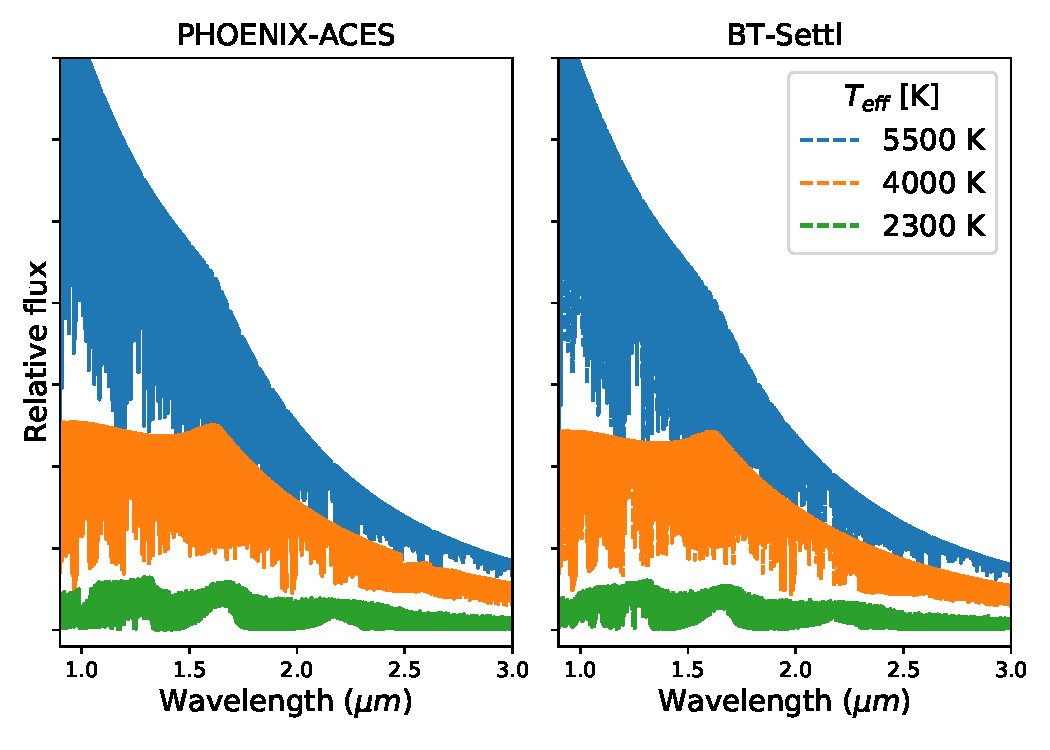
\includegraphics[width=0.5\linewidth]{figures/atmos_and_models/phoenix_large_scale_comparision}
    \caption[Large scale comparison between the {PHEONIX-ACES} and {BT-Settl} spectra.]{{PHOENIX-ACES} (left) and {BT-Settl} (right) spectra in the \nir{} wavelength region for three different temperature stars, \logg{}=4.5, \feh{}=0.}
    \label{fig:phoenixlargescalecomparision}
\end{figure}

\begin{figure}
    \centering
    \begin{tabular}{cc}
        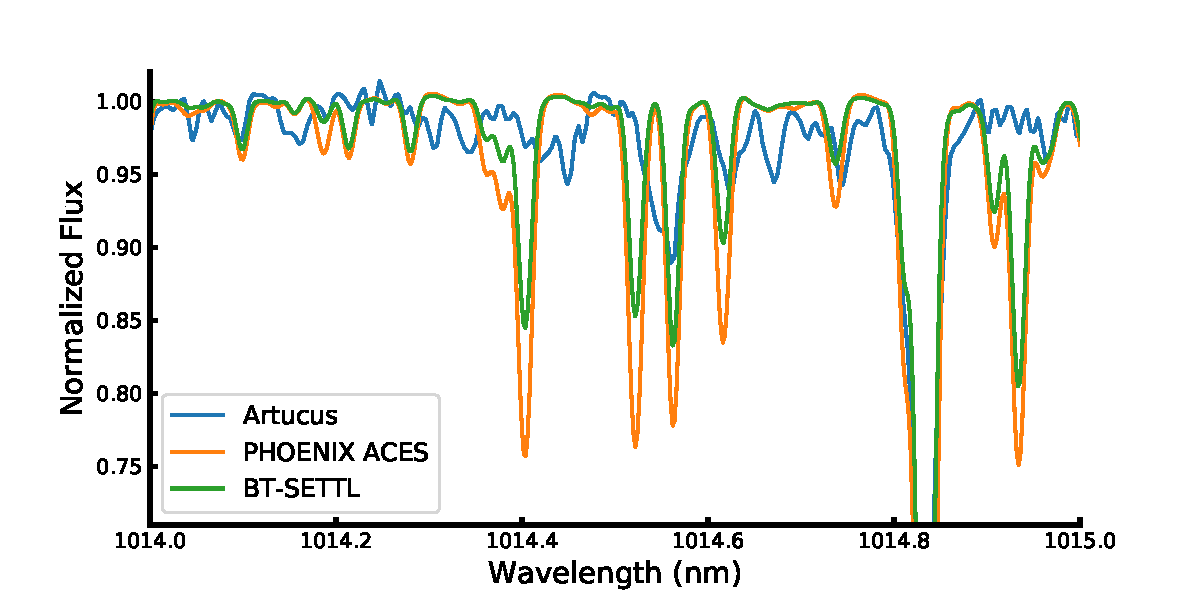
\includegraphics[width=0.48\linewidth]{figures/atmos_and_models/artucus_1micron} & 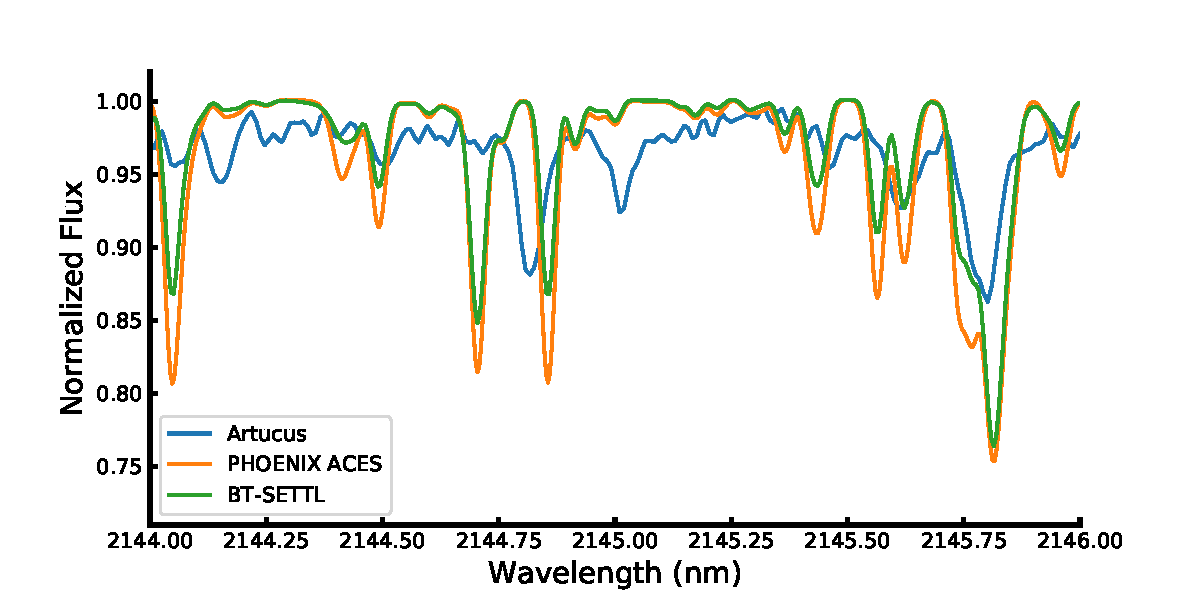
\includegraphics[width=0.48\linewidth]{figures/atmos_and_models/artucus_2micron}\\
    \end{tabular}
    \caption[Comparision of the spectrum of Arcturus to synthetic specta.]{Spectrum of Arcturus compared to synthetic spectra with the closest spectral parameters at wavelengths around 1014\nm{} (left) and 2145\nm{} (right).}
    \label{fig:artucus1-2micron}
\end{figure}

Here a comparison between the {PHOENIX-ACES} and {BT-Settl} spectra is briefly given.
\Cref{fig:phoenixlargescalecomparision} shows the model spectral flux in the \nir{} range of 0.9--3\um{} for three different stellar temperatures: 5500, 4000, and 2300\K{}.
At this large scale the spectra look fairly similar.

On closer inspection though, the spectra are slightly different with the {PHOENIX-ACES} spectra having deeper absorption lines compared to the {BT-Settl} models; however they do appear to have most of the same absorption lines.
This can be seen in \cref{fig:artucus1-2micron} which contains the {PHOENIX-ACES} and {BT-Settl} at two different regions in the \nir, 1013\nm{} and 2110\nm{}.
Temperature of both models is 4300\K{} while the \logg{} is 1.5 for {PHOENIX-ACES} and 2.5 for {BT-Settl} (closest available) and the models are convolved to R=100,000.
This is in an attempt to match the parameters to the observations of {Arcturus} at R=100\,000 shown blue.
Cross-correlation and a Doppler shift has been used to align the model spectra to the observations.
There is a striking difference between the models and observations with several lines present in the models that are not seen in the real observation, while a few lines observed that are not seen in the models.
When the observed absorption lines do align with the models there is a difference in the depth of the lines.
These differences are shown at two different wavelengths and reveal that there is still room for improvement in the synthetic models to match observed spectra in the \nir{} and at high resolution.
Spectral decadencies in the {BT-Settl} models are noted by~\citet{rajpurohit_effective_2013}.

A further example of this is shown in \cref{fig:visualinspection-hd2118471} in which the fitted model, dominated by a single {PHOENIX-ACES} model, is compared to the observed {CRIRES} spectra.
This caused issues with the fitting procedure in \cref{cha:model_comparison}.
\Cref{fig:crires-pop-mismatch} is a further example of the spectral differences at the \nir{} wavelengths specifically used in this work, in a spectra from (in reduced form) the CRIRES-POP library~\citep{lebzelter_crirespop_2012,nicholls_crirespop_2017}.
It shows differences between the CRIRES-POP \emph{K}-band spectra of {10\,Leo} and the {PHOENIX-ACES} spectrum with corresponding parameters (\txteff=4800, \logg{}=3.00, \feh{}=0.0).


\begin{figure}
    \centering
    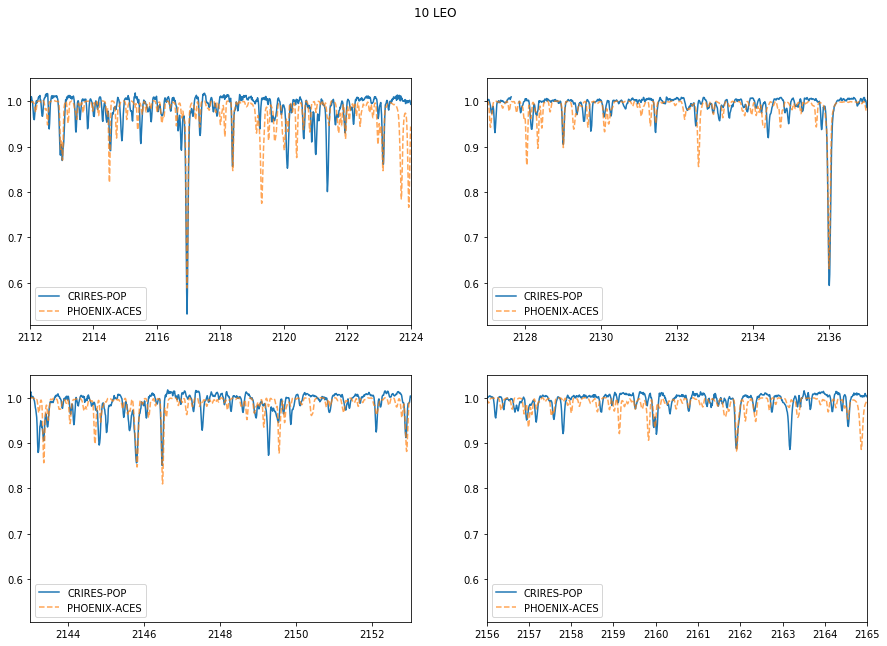
\includegraphics[width=0.7\linewidth]{figures/atmos_and_models/CRIRES-POP-mismatch}
    \caption[Comparision of the spectrum of {10\,Leo} to synthetic {PHOENIX-ACES} spectum.]{CRIRES-POP spectra of {10\,Leo} compared for {PHOENIX-ACES} model for the wavelength range setting used in \cref{cha:direct_recovery,cha:model_comparison}.}
    \label{fig:crires-pop-mismatch}
\end{figure}
\todo{\cref{fig:crires-pop-mismatch} needs improved style}




\subsection{Differential techniques}
\todo{ maybe this should go in differential chapter}
See \citet{kostov... 2013} for lots of useful references regarding differential works Simon and Sturm 1994

Rodler 2012 uses differential of a series of phases to construct a stellar mask for the host to subtract from all measurements.
